\chapter{Numerical Methods}\label{ch:numericalMethods}

%\emph{With the help of computers, very complex partial differential equations can be solved using finite element methods. By refining the mesh size the accuracy can be improved, However, this gained accuracy comes with a price. The more accurate the result is going to be to more computationally expensive the calculation will be.}

\section{Introduction}
With the development of high-speed computers as well as advances in numerical algorithms, numerical solution methods became a new tool to solve problems for a wide range of engineering disciplines, such as civil, mechanical, electrical and chemical engineering~\cite{Martin1973,Reddy1993}. In fact, numerical solutions methods are playing an ever-increasing role as a research and design tool, as well as helping to interpret and understand the results of theory and experiment, and vice versa.
%However, to work with numerical solutions, a solid background in both, the physics and numerical analysis, is needed. 

Similar to a theoretical approach, numerical analysis firstly represents the problems by physical models. These physical models should then be interpreted as mathematical models by establishing the governing equations as well as the boundary and initial conditions. Different from theoretical analysis, to obtain an approximate solution numerically, numerical methods adopt a discretization method which substitutes the governing differential equations by a series of algebraic equations which can then be solved on a computer. In general, for mesh-based methods, the discretization process divides the whole domain into small sub-domains in space and time, so the solution derived above is actually a numerical solution which applies to discrete locations. Thus, the accuracy of the solution is dependent on the quality and fineness of discretization, amongst other things.

The work throughout this project has made extensive use of finite element analysis (FEA) to model the magnetic field. FEA is especially useful for calculating the magnetic fields because analytical expressions for magnetic fields are available for only the most simple geometries~\cite{Furlani2006}. The software package ANSYS Maxwell was used because it offers the possibility to model 3D geometries and is highly recognized throughout the industry. It uses the finite element method to numerically solve the discretized model. 

\section{Finite Element Method}\label{sec:finiteElementMethod}
The finite element method (FEM) is a numerical technique for obtaining approximate solutions of differential equations. It has evolved into one of the most powerful and widely used techniques for finding numerical solutions of partial differential equations that occur in engineering and science. The reason for the popularity of the FEM is due to its flexibility and its vast range of applications~\cite{Zienkiewicz1971,Strang1988,Rao2005}. 

The fundamental principle of the FEM is to break a continuous problem into a discrete physical representation consisting of a finite number of regions or finite elements. In each element the unknown function $\Phi$ is represented by an interpolation function $\tilde{\Phi}$ with unknown coefficients. Thus, the original differential equation problem with an infinite number of degrees of freedom is converted into a problem with a finite number of degrees of freedom, or in other words, the solutions of the entire system are approximated by a finite number of unknown coefficients. So the solution derived is actually a numerical solution which applies to discrete locations.

In order to derive the system of algebraic equations various approximate methods have been developed, and among them the Ritz variational method and Galerkin approximation method have been used most widely. ANSYS Maxwell uses the Ritz variational method which is why only this approach will be discussed here. A brief explanation to the Galerkin approximation can be found in the Appendix~\ref{sec:galerkinMethod} for the sake of completeness or in the literature~\cite{Jin2014}. 

\subsection{Domain discretization}
\label{subsec:domainDiscretization}
The discretization of the domain $\Omega$ is normally the first step in any FEA. One of the most commonly used approach for two-dimensional (2D) and three-dimensional (3D) problems, is to divide the domain into a mesh of triangles or tetrahedra, respectively. These basic building blocks, triangle or tetrahedral, are called elements and are depicted in Figure~\ref{fig:typicalFiniteElements}.

\begin{figure}[htb]
  \begin{minipage}[t]{0.48\textwidth}
  	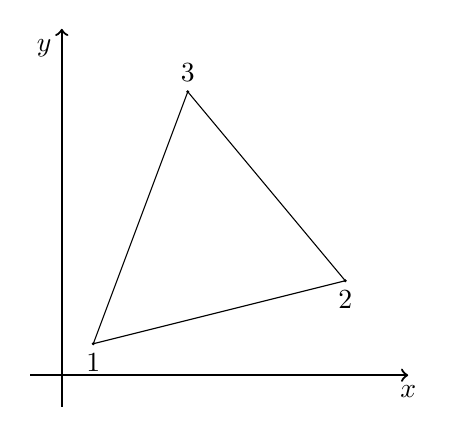
\begin{tikzpicture}[scale=0.4]
	\draw[thick,->] (-1,0)  -- (11,0) node[anchor=north] {$x$};
  	\draw[thick,->] (0,-1) -- (0,11) node[anchor=north east] {$y$};
  
  	\coordinate[label=below:$1$] 	(p1) at (1,1);
	\coordinate[label=below:$2$] 	(p2) at (9,3);
	\coordinate[label=above:$3$] 	(p3) at (4,9);
	
	\fill (p1) circle (1.5pt);
	\fill (p2) circle (1.5pt);
	\fill (p3) circle (1.5pt);
  
  	\draw (p1) -- (p2) -- (p3) -- cycle;
	\end{tikzpicture}
  \end{minipage}
  \hfill
  \begin{minipage}[t]{0.48\textwidth}
  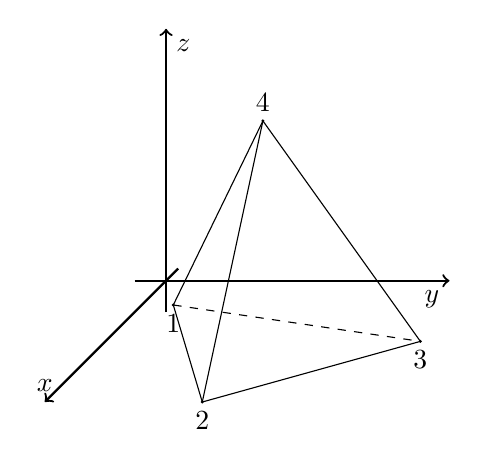
\begin{tikzpicture}[scale=0.4]
  \draw[thick,->] (-1,0,0) -- (9,0,0) node[thick,anchor=north east]{$y$};
  \draw[thick,->] (0,-1,0) -- (0,8,0) node[thick,anchor=north west]{$z$};
	\draw[thick,->] (0,0,-1) -- (0,0,10) node[thick,anchor=south]{$x$};
	
	\coordinate[label=below:$1$] 	(p1) at (1,0,2);
	\coordinate[label=below:$2$] 	(p2) at (5,0,10);
	\coordinate[label=below:$3$] 	(p3) at (10,0,5);
	\coordinate[label=above:$4$] 	(p4) at (5,7,5);
	
	\fill (p1) circle (1.5pt);
	\fill (p2) circle (1.5pt);
	\fill (p3) circle (1.5pt);
	\fill (p4) circle (1.5pt);
  
  \draw[solid] 	(p1) -- (p2);
  \draw[dashed] (p1) -- (p3);
  \draw[solid] 	(p2) -- (p3);
  \draw[solid] 	(p1) -- (p4);
  \draw[solid] 	(p2) -- (p4);
  \draw[solid] 	(p3) -- (p4);
  
	\end{tikzpicture} 
  \end{minipage}
  \caption[Typical finite elements: triangular element and tetrahedral element]{Typical finite elements: triangular element and tetrahedral element.}
  \label{fig:typicalFiniteElements}
\end{figure}

The mesh must satisfy nearly contradictory requirements: it must conform to the shape of the object or simulation domain; its elements may be neither too large nor too numerous; it may have to grade from small to large elements over a relatively short distance; and it must be composed of elements that are of the right shapes and sizes. The \textit{right} shapes typically include elements that are nearly equilateral and equiangular, and typically exclude elements that are long and thin, e.g. shaped like a needle or a kit~\cite{Cheng2012}.

ANSYS Maxwell employs multiple automated triangular meshing algorithms behind the scenes using default physics controls to ensure a high quality mesh suitable for the defined simulation. It also has an adaptive mesh refinement algorithm built in. After an initial coarse mesh has been generated, the number of elements will be increased in areas where fields are of interest or the field gradient or energy error is high. 

\subsection{Formulation of finite element equations for magnetostatic problems}
\label{subsec:formulation of finite element equations}
All macroscopic electromagnetic phenomena are governed by a set of equations, known as the Maxwell's equations. For the magnetostatic problem, where the magnetic field is time-invariant and the electric field can be neglected, the magnetic field must satisfy the following differential equations~\cite{Maxwell1873}:

\begin{eqnarray}
	\mathbf{\nabla} \times \mathbf{H} &=& \mathbf{J} \label{eqn:ampereLaw} \\
	\mathbf{\nabla} \cdot \mathbf{B} &=& 0 \label{eqn:gaussLaw} \\
	\mathbf{B} &=& \mu_{0}\mu_{r}\mathbf{H} \label{eqn:simpleLaw}
\end{eqnarray}

where $\mathbf{H}$, $\mathbf{B}$ and $\mathbf{J}$ are the magnetic field intensity, the magnetic flux density and the current density, respectively. The magnetic flux density can be expressed in terms of its vector potential $\Phi$:

\begin{equation}
	\mathbf{B} = \mathbf{\nabla} \times \Phi
	\label{eqn:magneticFluxVectorPotential}
\end{equation}

Substituting Equation~\ref{eqn:magneticFluxVectorPotential} into Equation~\ref{eqn:ampereLaw} with the aid of Equation~\ref{eqn:simpleLaw} yields the second-order differential equation:

\begin{equation}
	\mathbf{\nabla} \times \left(\frac{1}{\mu_{0}\mu_{r}}\nabla \times \Phi \right) = \mathbf{J}
	\label{eqn:vectorPotential}
\end{equation}

Assuming the magnetic permeability is isotropic and independent of the magnetic field, Equation~\ref{eqn:vectorPotential} can be written as Poisson's equation:

\begin{equation}
	\mathbf{\nabla}^{2} \Phi = \Delta \Phi = \mu_{0}\mu_{r}\mathbf{J} \text{ in } \Omega
	\label{eqn:vectorPotentialPoissonEquation}
\end{equation}

where $\Delta$ is the Laplace operator and the vector potential $\Phi$ needs to be a real function in the problem domain $\Omega$ with boundary $\partial \Omega$. This boundary value problem can be formulated as a variational expression (Ritz method), called \textit{functional}. ANSYS Maxwell uses the energy functional given by:

\begin{equation}
	E(\Phi) = \frac{1}{2}\int_{\Omega}\left(\frac{\nabla\Phi \cdot \nabla\Phi}{\mu_{0}\mu_{r}}+\Phi J\right)d\Omega
	\label{eqn:energyFunctional}
\end{equation}

However, the vector potential $\Phi$ in Equation~\ref{eqn:energyFunctional} is formulated as a continuous function, which FEM cannot deal with. Therefore, $\Phi$ will be replaced with a trial function $\tilde{\Phi}$, where the desired field in each element is approximated with a $2\textsuperscript{nd}$ order quadratic polynomial:

\begin{equation}
	\tilde{\Phi}(x,y,z) = a_{0}+a_{1}x+a_{2}y+a_{3}z+a_{4}xy+a_{5}yz+a_{6}xz+a_{7}x^{2}+a_{8}y^{2}+a_{9}z^{2}
	\label{eqn:basisFunction}
\end{equation}

The parameters $a_{i}$ are unknown values, which need to be found. In order to obtain these values, field quantities are calculated for 10 points of each element, shown in Figure~\ref{fig:finiteElementMethodPoints}. 

\begin{figure}[htb]
\centering
  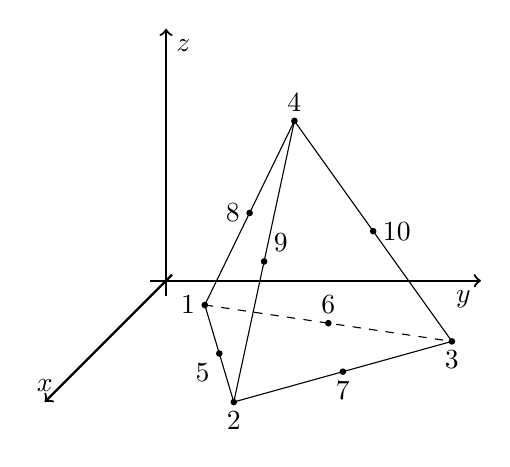
\begin{tikzpicture}[scale=0.4]
  \draw[thick,->] (-1.5,0,0) -- (9,0,0) node[thick,anchor=north east]{$y$};
  \draw[thick,->] (-1.0,-0.5,0) -- (-1.0,8,0) node[thick,anchor=north west]{$z$};
	\draw[thick,->] (-1.0,0,-0.5) -- (-1.0,0,10) node[thick,anchor=south]{$x$};
	
	\coordinate[label=left:$1$] 	(p1) at (1,0,2);
	\coordinate[label=below:$2$] 	(p2) at (5,0,10);
	\coordinate[label=below:$3$] 	(p3) at (10,0,5);
	\coordinate[label=above:$4$] 	(p4) at (5,7,5);
	\coordinate[label=below left:$5$] 	(p5) at (3,0,6);				
	\coordinate[label=above:$6$] 	(p6) at (5.5,0,3.5);
	\coordinate[label=below:$7$] 	(p7) at (7.5,0,7.5);
	\coordinate[label=left:$8$] 	(p8) at (3,3.5,3.5);
	\coordinate[label=above right:$9$] 	(p9) at (5,3.5,7.5);
	\coordinate[label=right:$10$] 	(p10) at (7.5,3.5,5);
		
	\fill (p1) circle (3pt);
	\fill (p2) circle (3pt);
	\fill (p3) circle (3pt);
	\fill (p4) circle (3pt);
	\fill (p5) circle (3pt);
	\fill (p6) circle (3pt);
	\fill (p7) circle (3pt);
	\fill (p8) circle (3pt);
	\fill (p9) circle (3pt);
	\fill (p10) circle (3pt);
  
  \draw[solid] 	(p1) -- (p2);
  \draw[dashed] (p1) -- (p3);
  \draw[solid] 	(p2) -- (p3);
  \draw[solid] 	(p1) -- (p4);
  \draw[solid] 	(p2) -- (p4);
  \draw[solid] 	(p3) -- (p4);
  
	\end{tikzpicture} 
  \caption[Interpolation points on a single element in FEM]{Points for which the magnetic vector potential will be calculated in the FEM. Field quantities inside the tetrahedral are calculated using a $2\textsuperscript{nd}$ order quadratic interpolation scheme.}
  \label{fig:finiteElementMethodPoints}
\end{figure}

The solution to these points, which obviously solves Equation~\ref{eqn:vectorPotentialPoissonEquation}, can then be obtained by minimizing the energy functional (Equation~\ref{eqn:energyFunctional}) with respect to the values $a_{i}$ and subject to the given boundary conditions and user defined initial conditions. Proof can be found in~\cite{Mikhlin1964}. This calculation is done at each node in every tetrahedral which results in a large, sparse matrix equation, which can be solved using standard matrix solution techniques, e.g. sparse Gaussian eliminator or incomplete Choleski conjugate gradient method.

\section{Error estimation of the finite element method}
\label{sec:errorEstimationOfTheFiniteelementMethod}
Even though FEM has evolved into one of the most widely used techniques for finding approximate solutions to differential equations it suffers from one major problem. The very act of subdividing the domain $\Omega$ provides the opportunity for \emph{discretization errors}. First, discretization errors occur because the \emph{finite} element model is, by definition, incapable of reproducing every one of the \emph{infinite} solution patterns that the problem domain can assume. Second, the construction of these subsets of the domain might result in a badly conditioned mesh, which negatively affects the solution of the individual elements~\cite{Cheng2012}. Therefore, not only the \emph{size} but also the \emph{qualtiy} of the mesh matters.

The discretization error $\epsilon$ is the difference between the true function $\Phi$ and its finite element approximation $\tilde{\Phi}$ in any given norm:

\begin{equation}
	\epsilon = \|\Phi - \tilde{\Phi}\|_{\star}
	\label{eqn:discretizationError} 
\end{equation}

Since this expression (Equation~\ref{eqn:discretizationError}) involves the exact but unknown solution $\Phi$ the error cannot exactly be measured but only estimated by lower and upper bounds. Such error estimations can be distinguished in \emph{a priori} and \emph{a posteriori} error estimations~\cite{Dow1998,Kunert1998}. 

%%%% This needs to be changed %%%%%%
\subsection{A priori error estimation}
\label{subsec:aPrioriErrorEstimation}
The \emph{a priori} error estimates the convergence of a given finite element method. Using the Cauchy$-$Schwarz inequality the following error estimates for Lagrange interpolation are known in the literature (see~\cite{Ciarlet1978,Brenner2008}). The following three norms, energy norm ($H_{1}$), p-norm $L_{p}$ and infinity or max norm ($L_{\infty}$), are mostly used in the literature:

\begin{eqnarray}
	\|\Phi - \hat{\Phi}\|_{H^{1}} &\leq & C\omega^{p}\|\Pi^{p+1}\Phi\|_{L_{2}} \label{eqn:energyNorm}\\
	\|\Phi - \hat{\Phi}\|_{L_{p}} &\le & C\omega^{p+1}\|\Pi^{p+1}\Phi\|_{L_{p}} \text{ with } 1 \leq p < \infty \label{eqn:pNorm}\\
	\|\Phi - \hat{\Phi}\|_{L_{\infty}} &\leq & C\omega^{p+1}\|\Pi^{p+1}\Phi\|_{L_{\infty}} \label{eqn:infinityNorm}
\end{eqnarray}

As it is standard in the finite element literature, the parameter $\omega$ describes the maximum length scale of all elements in the mesh, the parameter $C$ is a constant which is independent of $\omega$ and the solution $\Phi$, $p$ is the order of the interpolation function and $\Pi^{p+1}\Phi$ denotes the tensor of all derivatives of order $p+1$ of $\Phi$.

In the three norms, constant $C$ as well as the higher order derivatives of $\Phi$ are mostly unknown. Therefore, these estimates are largely theoretical. However, it can be seen that the error defined by these norms will with decreasing $\omega$ also decrease at the order of $O(\omega^{p})$ or $O(\omega^{p+1})$. Thus, the error will decrease much faster when using the quadratic method than when using the linear method, and the quadratic method is usually more efficient computationally speaking, but it also requires the function $\Phi$ to have three derivatives, whereas the error estimates for the linear method only require two derivatives. 

These estimates in the equations above (Equation~\ref{eqn:energyNorm}-\ref{eqn:infinityNorm}) are only valid if the mesh is regular. A regular mesh is achieved by keeping its aspect ratio $\theta$ below a positive constant $\vartheta$:

\begin{equation}
	\theta = \frac{\varrho_{out}}{\varrho_{in}} \leq \vartheta
\end{equation}

where $\varrho_{out}$ and $\varrho_{in}$ are the outer and inner diameter of the element (triangle or tetrahedral), respectively. If $\vartheta$ is small, normally $\vartheta\leq 5$ the mesh quality is considered to be sufficient.

The mesh quality not only affects the asymptotic behaviour of the solver it also influences the result. The literature also demonstrates that the accuracy of finite element solutions on triangular meshes degrades as angles are allowed to approach $180^{\circ}$~\cite{Babuska1976,Cheng2012}. Figure~\ref{fig:meshShape} visually illustrates these effects. The three triangulations are each using $200$ triangles to render a paraboloid. It can be seen that the mesh of Figure~\ref{fig:small}, where the mesh is composed by long thin triangles with no angle is greater than $90^{\circ}$, only performs slightly worse than the isotropic triangulation in Figure~\ref{fig:normal}. However, when the angles approach $180^{\circ}$ as shown in Figure~\ref{fig:large}, the solution gets more distorted. 

\begin{figure}[htb]
        \centering
        \begin{subfigure}[b]{0.3\textwidth}
                \includegraphics[width=\textwidth]{img/chapters/numericalMethods/normalAngleResult.eps}
        \end{subfigure}
        \begin{subfigure}[b]{0.3\textwidth}
                \includegraphics[width=\textwidth]{img/chapters/numericalMethods/smallAngleResult.eps}
        \end{subfigure}
        \begin{subfigure}[b]{0.3\textwidth}
                \includegraphics[width=\textwidth]{img/chapters/numericalMethods/largeAngleResult.eps}
        \end{subfigure}
        \begin{subfigure}[b]{0.3\textwidth}
                \includegraphics[width=\textwidth]{img/chapters/numericalMethods/normalAngleMesh.eps}
                \caption{}
                \label{fig:normal}
        \end{subfigure}
        \begin{subfigure}[b]{0.3\textwidth}
                \includegraphics[width=\textwidth]{img/chapters/numericalMethods/smallAngleMesh.eps}
                \caption{}  
                \label{fig:small}              
        \end{subfigure}
        \begin{subfigure}[b]{0.3\textwidth}
                \includegraphics[width=\textwidth]{img/chapters/numericalMethods/largeAngleMesh.eps}
                \caption{}                
                \label{fig:large}
        \end{subfigure}
        \caption[Illustration how large angles in element negatively effect FEM results]{Visual illustration of how large angles negatively effect the result of the FEM. In each triangulation, 200 triangles are used to render the 2D parabolic function.}
        \label{fig:meshShape}
\end{figure}

\subsection{A posteriori error estimation}
\label{subsec:aPosterioriErrorEstimation}
Having computed a finite element solution, it is possible to obtain \emph{a posteriori} error estimates. These estimates accomplish two main goals. Firstly, they are able to numerically quantify the actual error. Secondly, they can be used to perform \emph{adaptive mesh refinement}. Adaptive mesh refinement solves the problem iteratively. The method uses \emph{a posteriori} error estimators to indicate where errors are particularly high, and more mesh intervals are then placed in those locations. This process can be repeated until a satisfactory error tolerance is reached. 

As seen in Section~\ref{subsec:aPrioriErrorEstimation} the accuracy of the FEM solution highly depends on the element size as well as the $\Pi^{p+1}\Phi$ derivative. In the case where $\tilde{\Phi}$ is the quadratic approximation of $\Phi$, the error depends on the change of curvature of $\Phi$. Therefore, more mesh points should be placed in areas where the change of curvature is largest, in order to minimize the discretization error. However, neither the function $\Phi$ nor its third derivative $\Phi'''$ are exactly known, which makes it impossible to know where to place mesh points before computing a finite element solution. Thus, an adaptive mesh refinement scheme is used. Multiple adaptive mesh refinement algorithms using different \emph{a posteriori} error estimators are described in the literature to overcome this problem~\cite{Ainsworth2011,Verfurth1994,Verfurth2013}. Babu\v{s}ka et al. developed a refinement method where more mesh points are placed in areas where the gradient of the solution is highest~\cite{Babuska1978,Babuska1978_2,Babuska1979,Babuska1981}. Alternatively, one could refine the mesh according to the jump in the derivative at the element boundaries~\cite{Zienkiewicz1987}. Another approach, which will be used in this thesis, is using the residual $\varepsilon_{e}$:

\begin{equation}
	\varepsilon_{e} = \Delta \tilde{\Phi} - \mathbf{J}
\end{equation}

The parameter $\varepsilon_{e}$ indicates how well the original equations are locally satisfied by the approximate solution~\cite{Zienkiewicz1983}. The generated mesh is required to meet acceptable energy error estimate:

\begin{equation}
	\xi_{e} = \frac{|\varepsilon_{e}|}{E(\tilde{\Phi})}
	\label{eqn:localPercentEnergyErrorEstimate}
\end{equation}

where $\xi_{e}$ is the local energy error in element $e$ and $E(\tilde{\Phi})$ describes the total energy in the discrete system, which for the FEM approximate solution can be formulated as the following (also see Equation~\ref{eqn:energyFunctional}):

\begin{equation}
	E(\tilde{\Phi}) = \frac{1}{2}\int_{\Omega}\left(\frac{\nabla \tilde{\Phi}\nabla \tilde{\Phi}}{\mu_{0}\mu_{r}}+\tilde{\Phi} J \right)d\Omega
	\label{eqn:totalEnergy}
\end{equation}

Recall that $\Phi$ is unknown, but the error can still be determined~\cite{Cendes1985}. The $\xi_{e}$ values act as an energy error estimate criteria and are used for adaptive mesh refinement. It has been shown by Babu\v{s}ka and Rheinboldt that if $\xi_{e}$ is equal for all elements, then the model using the given number of elements is the most efficient one. This concept is also referred to as \emph{error equilibration}~\cite{Babuska1979_2}.

Summing the local errors in each element and dividing the sum by the total energy leads to a global percentage error energy:

\begin{equation}
	\xi = \frac{\sum_{e=1}^{n}|r_{e}|}{E(\tilde{\Phi})}
	\label{eqn:globalPercentEnergyErrorEstimate}
\end{equation}

Equation~\ref{eqn:globalPercentEnergyErrorEstimate} is used as a stopping criteria in order to terminate the refinement process. 

\section{Finite element method validation}\label{sec:femValidation}
In order to evaluate the solution computed by ANSYS Maxwell a mesh independence study was performed, where the number of nodes in the mesh will be gradually increased until no significant change in the solution can be detected. This approach will be shown by using a simple bar magnet as a canonical example. This magnet geometry is used over the course of this work and thus conducting a grid independence analysis for this design has an application value.

The refinement of the mesh will be done by ANSYS Maxwell's built in adaptive mesh refinement algorithms, using different termination values for $\xi$, which has been described above (see Section~\ref{subsec:aPosterioriErrorEstimation}).

% maybe also element quality will be tested. 

\subsection{Grid independence study}
\label{subsec:gridIndependenceStudy}
Under the same discretization scheme, a significant portion of computational error, the discretization error, is related to the fineness of the mesh applied. If the mesh is fine enough so that the solution cannot be improved markedly by refining the grid any more, the solution is said to achieve grid independence. To guarantee that the computational solution is reliable and invariant to refinement of the mesh, a grid independence study is conducted. The schematic of the model used for this study is shown in Figure~\ref{fig:barMagnetScheme}.

\begin{figure}[htb]
\centering
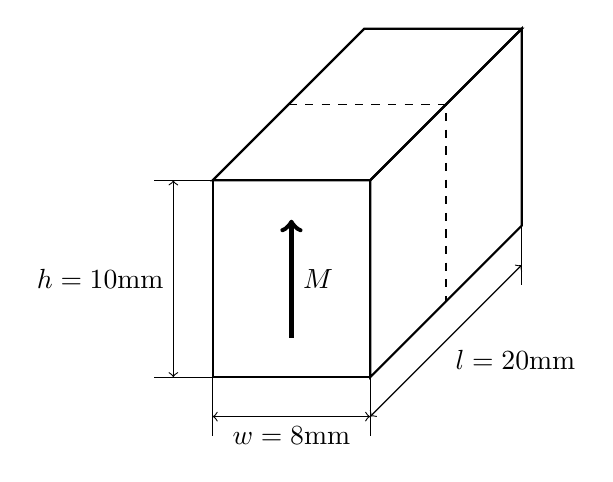
\begin{tikzpicture}[scale=1.0]
	\coordinate 	(A) at (0,0,0);
	\coordinate 	(B) at (2,0,0);
	\coordinate 	(C) at (2,2.5,0);
	\coordinate 	(D) at (0,2.5,0);
	\coordinate 	(E) at (0,0,5);
	\coordinate 	(F) at (2,0,5);
	\coordinate 	(G) at (2,2.5,5);
	\coordinate 	(H) at (0,2.5,5);
	\coordinate 	(P1) at (0,-0.75,5);		
	\coordinate 	(P2) at (2,-0.75,5);			
	\coordinate 	(P3) at (2,-0.75,0);
	\coordinate 	(P4) at (-0.75,0,5);	
	\coordinate 	(P5) at (-0.75,2.5,5);	
	\coordinate 	(P6) at (1,0.5,5);
	\coordinate 	(P7) at (1,2,5);	
	
	\coordinate 	(P8) at (0,2.5,2.5);
	\coordinate 	(P9) at (2,2.5,2.5);
	\coordinate 	(P10) at (2,0,2.5);
	\coordinate 	(P11) at (0,0,2.5);

	
	\draw[thick] (E) -- (F) -- (G) -- (H) -- cycle;
	\draw[thick] (D) -- (C) -- (G) -- (H) -- cycle;
	\draw[thick] (B) -- (C) -- (G) -- (F) -- cycle;
	\draw (E) -- (P1);
	\draw (F) -- (P2);	
	\draw (B) -- (P3);
	\draw (E) -- (P4);
	\draw (H) -- (P5);	
	\draw[<->] (0,-0.5,5) -- node[below]{$w=8$mm} (2,-0.5,5);
	\draw[<->] (-0.5,0,5) -- node[left]{$h=10$mm} (-0.5,2.5,5);
	\draw[<->] (2,-0.5,5) -- node[below right]{$l=20$mm} (2,-0.5,0);
	\draw[line width=1.8pt,->] (P6) -- node[right]{$M$}(P7);
	
	\draw[dashed] (P8) -- (P9) -- (P10);
\end{tikzpicture}
\caption[Bar magnet schematic]{Bar magnet schematic. Vector $M$ shows the direction of the magnetization. The dashed line indicates the centre plane through the middle of the magnet. }%
\label{fig:barMagnetScheme}%
\end{figure}

In this study, four different global percentage errors of the total energy are used as a termination criteria. The corresponding mesh densities for the four different values are shown in Figure~\ref{fig:meshPass} (a)-(c). The triangular grids in Figure~\ref{fig:meshPass} are plotted on a plane cut through the middle of the magnet, which is indicated by the dashed line in Figure~\ref{fig:barMagnetScheme}. The shaded area in Figure~\ref{fig:meshPass} highlights the cross section of the magnet. 

\begin{figure}[htb]
        \centering
        \begin{subfigure}[b]{0.47\textwidth}
                \includegraphics[width=\textwidth]{img/chapters/numericalMethods/meshPass1.eps}
                \caption{}
                \label{fig:meshPass1}
        \end{subfigure}
        \begin{subfigure}[b]{0.47\textwidth}
                \includegraphics[width=\textwidth]{img/chapters/numericalMethods/meshPass5.eps}
                \caption{}
                \label{fig:meshPass5}
        \end{subfigure}
        \begin{subfigure}[b]{0.47\textwidth}
                \includegraphics[width=\textwidth]{img/chapters/numericalMethods/meshPass10.eps}
                \caption{}
                \label{fig:meshPass10}
        \end{subfigure}
        \begin{subfigure}[b]{0.47\textwidth}
                \includegraphics[width=\textwidth]{img/chapters/numericalMethods/meshPass14.eps}
                \caption{}
                \label{fig:meshPass14}
        \end{subfigure}
        \caption[FEM unstructured mesh at the magnet's centre plane]{Mesh structure at the centre plane of the magnet ($z=0$) for different termination parameters $\xi$. (a) $\xi=10\%$. (b) $\xi=1\%$. (c) $\xi=0.1\%$. (d) $\xi=0.01\%$.}
        \label{fig:meshPass}
\end{figure}

It can be seen how the mesh density changes, especially around the corners where the change in the magnetic field is the largest and thus, energy errors are highest. In Figure~\ref{fig:magFieldPass} the magnetic $\mathbf{B}$ fields for the different mesh density are plotted and it can be seen how the accuracy of the solution improves with an increasing number of elements. Whereas the solution of the coarse grid (Figure~\ref{fig:magFiledPass1}) still looks very distorted, shows the last plot (Figure~\ref{fig:magFieldPass14}) a very smooth and continuous solution. Figure~\ref{fig:magFieldPass10} and Figure~\ref{fig:magFieldPass14}, however, lead to practically identical results and thus confirm grid independence. 

\begin{figure}[htb]
        \centering
        \begin{subfigure}[b]{0.47\textwidth}
                \includegraphics[width=\textwidth]{img/chapters/numericalMethods/magFieldPass1.eps}
                \caption{}
                \label{fig:magFiledPass1}
        \end{subfigure}
        \begin{subfigure}[b]{0.47\textwidth}
                \includegraphics[width=\textwidth]{img/chapters/numericalMethods/magFieldPass5.eps}
                \caption{}
                \label{fig:magFieldPass5}
        \end{subfigure}
        \begin{subfigure}[b]{0.47\textwidth}
                \includegraphics[width=\textwidth]{img/chapters/numericalMethods/magFieldPass10.eps}
                \caption{}
                \label{fig:magFieldPass10}
        \end{subfigure}
        \begin{subfigure}[b]{0.47\textwidth}
                \includegraphics[width=\textwidth]{img/chapters/numericalMethods/magFieldPass14.eps}
                \caption{}
                \label{fig:magFieldPass14}
        \end{subfigure}
        \caption[FEM magnetic flux density result at the magnet's centre plane]{Magnetic flux density magnitude for different termination parameters $\xi$. (a) $\xi=10\%$. (b) $\xi=1\%$. (c) $\xi=0.1\%$. (d) $\xi=0.01\%$.}
        \label{fig:magFieldPass}
\end{figure}

%In Figure~\ref{fig:magFieldPass} some errors have also been introduced since the solution has to be interpolated between the grid points. However, with increasing number of elements these errors will be more and more negligible. 

In Figure~\ref{fig:magFieldPass} some errors might have been introduced since the FEM solution was exported on a regular grid into MATLAB where some points needed to be interpolated. However, with increasing number of elements these errors will become negligible. 

The propagation of the percentage energy error can also be plotted against the number of elements in the mesh. Figure~\ref{fig:energyErrorAnsysMaxwell} shows how the energy error decreases with an increasing number of elements. 
%Even at a high number of elements, the error can still be marginally decreased. 

\begin{figure}[htb]
  \centering
      \includegraphics[width=0.7\textwidth]{img/chapters/numericalMethods/energyErrorAnsysMaxwell.eps}
  \caption[Percentage energy error in finite element system]{Percentage energy error in the model decreases with increasing number of nodes in the mesh. Even at higher number of elements, the error still drops.}
  \label{fig:energyErrorAnsysMaxwell}
\end{figure}

Based on the grid independence study, it becomes evident that the two finer grids result in the same solution. This suggests a percentage energy error of $\xi=0.1\%$. Adding a margin to this energy error, it suggests to use a termination error of $\xi=0.05\%$, which therefore will be used as termination criteria throughout this thesis.

All subsequent computations are also verified for grid independence, but for brevity evidence of this fact will not be presented.

\subsection{Mesh quality study}
\label{subsec:meshQualityStudy}
As seen previously not only the mesh density but also the mesh quality matters (see Section~\ref{subsec:aPrioriErrorEstimation}). Unfortunately, ANSYS Maxwell only provides very limited mesh statistics. Therefore, a customized MATLAB program was written, in order to calculate the regularity of the used mesh. 

At a percentage energy error of $0.1\%$ or smaller a highly regular mesh is achieved with a mean aspect ratio of $\bar{\theta}=4.6$ and a standard deviation of $\sigma_{\theta}=1.1$. Whereas for higher percentage energy errors ($\xi=10\%$) the aspect ratio and standard deviation also increases to $\bar{\theta}=87.5$ and $\sigma_{\theta}=30.2$, respectively. At these aspect ratio values the mesh can no longer be assumed to be regular, which degrades the accuracy of the computed solution (see Section~\ref{subsec:aPrioriErrorEstimation}).

\subsection{Experimental measurements}
\label{subsec:experimentalMeasurements}
It can be seen that the two sets of grids in Figure~\ref{fig:meshPass10} and Figure~\ref{fig:meshPass14} produce very reliable and meaningful solutions, while the coarser grids (Figure~\ref{fig:meshPass1} and Figure~\ref{fig:meshPass5}) lead to discrepancies which make the solution distinct from the real magnetic field pattern. This can be proven in many cases when comparing to the experimental data. 

%% this paragraph is used in experiments
Therefore, the magnetic flux density of the bar magnet was physically measured using a hand-held Hall sensor (5170 Gauss/Tesla Meter, F.W. Bell). The Hall sensor is constructed from a thin sheet of conductive material with output connections perpendicular to the direction of current flow. When subjected to a magnetic field, it responds with an output voltage proportional to the magnetic flux density.

The flux density of the bar magnet was measured at different distances away from the magnet surface, keeping the angle position of the Hall probe perpendicular to the flux lines in order to maximise the output signal. Figure~\ref{fig:magneticFluxDensitySimulationVsMeasurement} shows the comparison of the decreasing magnetic field with respect to the distance between the experimental measurements and the ANSYS Maxwell simulations. The numerical simulations match the experimental results with a maximum discrepancy of $12\%$; which, due to the size of the probe and positioning tolerance, is within the measurement error.

\begin{figure}[htb]
        \centering
        \begin{subfigure}[b]{0.47\textwidth}
                \includegraphics[width=\textwidth]{img/chapters/numericalMethods/magneticFluxDensitySimulationVsMeasurementParallel.eps}
                \caption{}
                \label{fig:magneticFluxDensityParallel}
        \end{subfigure}
        \begin{subfigure}[b]{0.47\textwidth}
                \includegraphics[width=\textwidth]{img/chapters/numericalMethods/magneticFluxDensitySimulationVsMeasurementPerpendicular.eps}
                \caption{}
                \label{fig:magneticFluxDensityPerpendicular}
        \end{subfigure}
        \caption[Measured magnetic flux density of a bar magnet]{Magnetic flux density at different distances away from the bar magnet's surface. The two plots show the measurement in (a) parallel and (b) perpendicular magnetization orientation.}
        \label{fig:magneticFluxDensitySimulationVsMeasurement}
\end{figure}


\section{Numerical magnetic force calculation}\label{sec:numericalMagneticForceCalcualtion}
As shown in the previous sections the solution for the magnetic field can be accurately estimated using FEM. The solution of the FEM has been exported onto a regular equispaced grid for further processing. The distance between neighbouring sample points was kept fixed in all directions and was chosen to be the size of the smallest element of the mesh in order to capture the FEM result accurately. Values of grid points which did not fit on the mesh directly, were interpolated using a second order polynomial interpolation method.

In order to numerically calculate the magnetic driving force, the derivative of the FEM results was taken by applying the forward numerical differencing approximation~\cite{Burden2001}

\begin{equation}
 	\mathbf{B}'(x) \approx \frac{\mathbf{B}(x+\omega)-\mathbf{B}(x)}{\omega}
 	\label{eqn:nummericalDifferentiation}
\end{equation} 

Unlike continuous functions, where $\omega\rightarrow 0$, the parameter $\omega$ is a small but positive number ($h>0$). This causes the force to be no longer a smooth function, but irregularities occur due to finite differentiation, as shown in Figure~\ref{fig:magnetophoreticMobilityBarMagnetNoise}. This negative effect is highly interconnected with the mesh size of the FEM. The finer the mesh, the less irregularities occur when the magnetic field is differentiated. However, with an increasing number of vertices the computational complexity increases. The theoretical run time to solve the partial differential equations (PDE) increases exponentially with an increasing number of elements, which is a disincentive~\cite{Johnson2004}.

\begin{figure}[htb]
        \centering
        \includegraphics[width=0.7\textwidth]{img/chapters/numericalMethods/magnetophoreticMobilityBarMagnetNoise.eps}
        \caption[Numerical magnetophoretic driving force]{The magnetophoretic driving force suffers from numerical irregularities due to the finite differentiation of the magnetic flux density.}
        \label{fig:magnetophoreticMobilityBarMagnetNoise}
\end{figure}

These irregularities, however, can also be reduced by applying a smoothing algorithm. Smoothing attempts to reduce the noise while capturing the important patterns in the data. In recent years smoothing has become a lot more prominent in different areas of computational science such as image recognition~\cite{Jain1989}, quantitative financial applications~\cite{Gencay2001} and big data analysis~\cite{Kantardzic2011}. 

In this work, smoothing is used to \textit{iron out} the numerical errors after the numerical differentiation of the simulated magnetic field on a three dimensional equispaced grid. Similar smoothing problems have already been solved mainly in image processing for noisy 2D images using different methods, e.g. kernel smoothing, adaptive smoothing (also Laplace smoothing) or total variation denoising~\cite{Jain1989,Buades2005}. The same approach can also be used for smoothing problems on a three dimensional grid, with only minor adjustments~\cite{Eubank1999,Takezawa2005}.

However, even if multiple smoothing algorithms are available, it is important to asses whether or not the chosen approach is appropriate. Therefore, the goodness of fit needs to be tested against some useful statistical standards. Additionally, the accuracy of the smoothing needs to be known. In other words, the likelihood of the errors of the fitted curve is of great interest. Finally, it is not uncommon in smoothing data, to discover that the performance of the smoothing algorithm is also model dependent. In some cases, one method might achieve a better result in some corner of the parameter space than others, but miss out on a lot of detail in other areas and vice versa. 

Therefore, in the following the different smoothing methods will be explained and compared with each other. Every proposed algorithm will be tested according to its goodness of fit.

%% Kernel Smoothing %%
\subsection{Kernel smoothing}\label{subsec:kernelSmoothing}
A kernel smoother is an intuitive estimate of a regression function. At each point $X_{i}$ the estimate is a locally weighted mean of the sample points $Y_{i}$. Given the kernel function $K$ the estimator $\hat{Y}$ can be described as~\cite{Nadaraya1964,Watson1964}:

\begin{equation}
	\hat{Y}_{i} = \frac{\sum_{j=1}^{N}{K(x-X_{j})Y_{j}}}{\sum_{i=j}^{N}K(x-X_{j})}
\label{eq:nadarayaWatsonKernel}
\end{equation}

The kernel function $K$ is a weighting function and gives different weights to the observations close to $X_{j}$. Additionally $K$ needs to be continuous, bounded and a symmetric real function which integrates to one:

\begin{equation}
	\int{K(u)du}=1
\label{eq:kernelCondition}
\end{equation}

%Unfortunately, this simplicity has flaws. At the boundary of the predictor space, their kernel neightborhood is asymmtric and the stimate may have substantial bias. Bias can be a problem in the interior as well if the predictor are nonuniform or if the regression function has substantial curvature. These problems are particularly sever when the predictors are multidimensional~\cite{} %Local Regression Automatic Kernel Carpentry

% Non-parametric regression is widely used in many scientific and engineering areas, such as image processing and pattern recognition.

\subsubsection{Moving average filter}
The moving average filter is the most typical technique for smoothing equispaced data. If the weights of the kernel are chosen to be all similar a moving average filter results. The resulting estimates can then be written as:

\begin{equation}
	\hat{Y}_{i} = \frac{1}{W}\sum_{j=1}^{W}Y_{j} 
\label{eq:movingAverageKernel}
\end{equation}  

where $W$ is the number of adjacent points of $x$ in the span, frame or box for a 1D, 2D or 3D problem, respectively. The smoothing depends on the size of this moving window. A wide moving window results in a less variable, more smooth fit, but it makes the estimator less responsive to local features as shown in Figure~\ref{img:movingAverage}.

\begin{figure}[htb]
   \centering   
   \includegraphics[width=0.7\textwidth]{img/chapters/smoothing/movingAverageFilterDifferentWindowSize.eps}
   \caption[Moving average filter smoothing]{Smoothing of a noisy sinusoidal curve using a moving average filter with different bandwidths. The sinusoidal curve has been interfered with Gaussian noise with mean 0, a standard deviation of 1 and an amplitude of 0.1}
   \label{img:movingAverage}
\end{figure}   

The objective is to choose the bandwidth in such a way that the variance will be reduced and the main features remain. Unfortunately, the two properties are negatively correlated. That is why it is always a trade-off between accuracy and smoothness.

\subsubsection{Gaussian filter}
Smoothing using a moving average is a very simple variation, where only the data points in the moving window have an influence on the average, while the remaining data receive no attention. Therefore, a different kernel can be defined, where the weights are Gaussian distributed:

\begin{equation}
	K = \frac{1}{\sqrt{2\pi\sigma^2}}\text{exp}\left(-\frac{x^2}{2\sigma^2}\right)
\label{eq:gaussianFilterKernel}
\end{equation}

where $x$ and $\sigma$ are the input data and standard deviation, respectively. Figure~\ref{img:gaussianFilter} depicts the Gaussian filter for different $\sigma$.

\begin{figure}[htb]
   \centering   
   \includegraphics[width=0.7\textwidth]{img/chapters/smoothing/gaussianFilter.eps}
   \caption[Gaussian filter smoothing]{Smoothing of a noisy sinusoidal curve using a Gaussian filter with different $\sigma$. The sinusoidal curve has been interfered with Gaussian noise with mean 0, a standard deviation of 1 and an amplitude of 0.5.}
   \label{img:gaussianFilter}
\end{figure}  

\subsubsection{Savitzky$-$Golay filter}
A much better procedure than simply averaging points is to perform a least squares fit of a small set of consecutive data points to a polynomial and take the calculated central point of the fitted polynomial curve as the new smoothed data point. Savitzky and Golay showed that a set of integers ($C_{-k}, a_{-(k+1)}, \cdots, a_{k-1}, a_{k}$) could be derived and used as weighting coefficients to carry out the smoothing operation~\cite{Savitzky1964}. The use of these weighting coefficients, known as convolution integers, are exactly equivalent to fitting the data to a polynomial. The smoothed data points $\hat{Y}$ are given by the following equation:

\begin{equation}
	\hat{Y}_{i} = \sum\limits_{j=-k}^{k}{C_{j}Y_{i+j}}
\label{eq:savitzkyGolayFilter}
\end{equation} 

where the parameters $C_{j}$ are the convolution coefficients and $k$ is an integer describing the size of the subset. Savitzky and Golay have published tables of convolution coefficients for various polynomials and sub-set sizes. 

The smoothing effect of the Savitzky-Golay algorithm is not so aggressive as in the case of the moving average and the loss or distortion of vital information is comparatively limited. The smoothing results of a Savitzky-Golay filter for  different sub-set sizes on a sinusoidal function is shown in Figure~\ref{fig:savitzkyGolayFilter}. It can be seen that already a sub-set order of five produces good results. 
% check references in MATLAB documentation and sgsf method and 'Comments on the Savitzky-Golay Convolution Method for Least-Squares Fit Smoothing and Differentiation of Digital Data'

\begin{figure}[htb]
   \centering   
   \includegraphics[width=0.7\textwidth]{img/chapters/smoothing/savitzkyGolayFilter.eps}
   \caption[Savitzky$-$Golay filter smoothing]{Smoothing of a noisy sinusoidal curve using a Savitzky-Golay filter with different polynomial order. The sinusoidal curve has been interfered with Gaussian noise with mean $0$, a standard deviation of $1$ and an amplitude of 0.5.}
   \label{fig:savitzkyGolayFilter}
\end{figure} 

%% Anisotropic diffusion
\subsection{Anisotropic diffusion}\label{subsec:anisotropicDiffusion}
In image processing and computer vision anisotropic diffusion (AD) is a technique aiming at reducing image noise without removing significant parts of the image content, typically edges, lines or other details that are important for the interpretation of the image. Perona and Malik proposed varying the conduction spatially to favour noise removal in nearly homogeneous areas while avoiding any alteration of the signal along significant discontinuities~\cite{Perona1990}. The AD is a nonlinear filtering operation which uses an iterative process. For each iteration, the edges are detected by determining the image gradient and for each pixel one coefficient of diffusion, which depends on the gradient value, is calculated. For low values of gradient, the diffusion is authorized with a high diffusion coefficient, although, for a high value of gradient, the diffusion is limited by a weak coefficient. Thus, the Perona-Malik equation can be given by~\cite{Perona1990}:

\begin{equation}
	\frac{\partial Y}{\partial t} = c(x,t)\Delta Y + \nabla c \cdot \nabla Y
	\label{eqn:peronaMalikEquation}
\end{equation} 

where $c(\cdot)$ is the proposed diffusion function which controls the rate of diffusion at any point. The function $c(\cdot)$ is chosen such that it follows the gradient magnitude at each point. This restrains the diffusion process around edges in images and thus keeps main features of the underlying data.

Perona and Malik suggest the following two diffusion functions:

\begin{eqnarray}
	c_{1}(\nabla Y) &=& \text{exp}\left(-\left[\frac{\Vert \nabla Y \Vert}{\kappa}\right]^{2}\right) \label{eqn:fluxFunction1}\\
	c_{2}(\nabla Y) &=& \frac{1}{1+\left(\frac{\Vert \nabla Y \Vert}{\kappa}\right)^{2}} \label{eqn:fluxFunction2}
\end{eqnarray}

where $\kappa$ is a positive parameter which governs the trade-off between edge preservation and blurring. In this work, $\kappa$ is set to $0.25$.

Figure~\ref{fig:anisotropicDiffusion} shows the results of the anisotropic diffusion algorithm for both flux functions (Equation~\ref{eqn:fluxFunction1} and Equation~\ref{eqn:fluxFunction2}).

\begin{figure}[htb]
   \centering   
   \includegraphics[width=0.7\textwidth]{img/chapters/smoothing/anisotripicDiffusion.eps}
   \caption[Anisotropic diffusion smoothing]{Smoothing of a noisy sinusoidal curve using the anisotropic diffusion algorithm. The $\kappa$ parameter of the flux function is set to $0.25$ and the algorithm is iterated 6 times. The sinusoidal curve has been interfered with Gaussian noise with mean 0, a standard deviation of 1 and an amplitude of 0.5.}
   \label{fig:anisotropicDiffusion}
\end{figure} 

%% total Variation Denoising %%
\subsection{Total variation denoising}\label{subsec:totalVariationDenoising}
Total variation denoising also known as the total variation regulation is an effective filtering method for recovering piecewise-constant signals, whilst preserving important details in the underlying signal. Total variation (TV) has been introduced in computer vision first by Rudin et al. as a regularizing criterion for solving inverse problems~\cite{Rudin1992}. 

Unlike a conventional low-pass filter (e.g. moving average filter), TV denoising is defined in terms of an optimization problem. The output of the TV denoising filter is obtained by minimizing the following cost function:

\begin{equation}
	\psi(\hat{Y}) = \frac{1}{2}\sum_{i=0}^{k-1}{(Y_{i}-\hat{Y}_{i})^2+\lambda \sum_{i=1}^{k-1}{|\hat{Y}_{i}-\hat{Y}_{i-1}|}}
\label{eq:totalVarianceCostFunction}
\end{equation}

The regularization parameter $\lambda$ is a real positive scalar that controls the degree of smoothing. In this work, the parameter $\lambda$ is determined by minimizing the generalized cross-validation (GCV) score.

The first term on the right-hand side reflects the expectation that the values of the data should be close to those of the estimates. This aim is common for that of the use of ordinary least square. The second term imposes the condition that the estimates should vary smoothly. This second term is called the roughness penalty. Using the cost function described in Equation~\ref{eq:totalVarianceCostFunction} the optimization problem can be formulated as:

\begin{equation}
	\arg\min_{\hat{Y}} \left\{ \psi(\hat{Y}) = \frac{1}{2}\sum_{i=0}^{k-1}{(Y_{i}-\hat{Y}_{i})^2+\lambda \sum_{i=1}^{k-1}{|\hat{Y}_{i}-\hat{Y}_{i-1}|}} \right\}
\label{eq:totalVarianceOptimizationProblem}
\end{equation}

This minimization problem (Equation~\ref{eq:totalVarianceOptimizationProblem}) is non-differentiable because of the $l_{1}$-norm. Numerous approaches have been developed to minimize the non-convex target function $\psi(\hat{Y})$. Chambolle~\cite{Chambolle1997,Chambolle2004,Chambolle2005} used an algorithm based on the dual formulation and the related work of Chan et al.~\cite{Chan2001,Chan2005,Chan2006}. Another simple and straightforward approach to express the cost function is by replacing the non-differentiable $l_{1}$-norm with a square integral of the $p^{\text{th}}$ derivative: % of $m(x)$: 
 
\begin{equation}
	\psi(\hat{Y}) = \frac{1}{2}\sum_{i=0}^{k-1}{(Y_{i}-\hat{Y}_{i})^2}+\lambda \int_{\hat{Y}_{1}}^{\hat{Y}_{k}}{\left(\frac{\partial^{p}\hat{Y}(t)}{\partial t^{p}}\right)^{2}dt}
\label{eq:smoothingSpline}
\end{equation}

This approach is known in the literature as smoothing spline~\cite{Takezawa2005, Wahba1990, Schoenberg1964}. In the remainder of this thesis the order of derivation will be restricted to $p=2$ (Whittaker-Henderson smoothing), which is used in most previous approaches~\cite{Whittaker1922, Spoerl1937, Spoerl1941, Joseph1952, Eilers2003} and will also be used in this thesis.

The objective function can then be expressed as:

\begin{equation}
	\psi(x) = \frac{1}{2}\sum_{i=0}^{k-1}{(Y_{i}-\hat{Y}_{i})^2}+\lambda \Pi \hat{Y}
	\label{eq:whittakerHendersonSmoothing}
\end{equation}

where the matrix $\Pi$ is defined as:

\begin{equation}
	\Pi = 
	\begin{bmatrix}
		-1 & 1 & & &\\
		1 & -2 & 1 & & \\
		& \ddots & \ddots & \ddots & \\
		& & 1 & -2 & 1 \\
		& & & 1 & 1
	\end{bmatrix}
\label{eq:}
\end{equation}

\subsection{Smoothing algorithm comparison}\label{subsec:smootingAlgorithmComparison}
All the different smoothing algorithms have been tested and compared by using the following 3D function:

\begin{equation}
	f(x,y) = x\cdot \text{exp}\left(-x^{2}-y^{2}\right)
	\label{eqn:testFunctionBump}
\end{equation}

This function was chosen, because it is a smooth and continuous function, which exhibits similar characteristics to the magnetic driving force distribution. Therefore, Equation~\ref{eqn:testFunctionBump} can be well used as a canonical smoothing process. Additionally, the exact results of Equation~\ref{eqn:testFunctionBump} can be determined and compared to the outcome of the smoothing algorithms. The residual sum of squares (RSS) was chosen as a quality measure to decide how well the smoothing data presents the original function. Figure~\ref{fig:smoothingAlgorithmComparisonOrigin} shows the results of the clean model and the noisy model. The noise was applied by superimposing random numbers whose elements are normally distributed with a mean $0$ and a standard deviation of $1$. The magnitude of the white noise was set to $0.1$.

\begin{figure}[htb]
\centering
	\begin{subfigure}[b]{0.47\textwidth}
		\includegraphics[width=\textwidth]{img/chapters/smoothing/smoothData2Dclean.eps}
		\caption{Clean data.}
    \end{subfigure}
    %%%%%%%%%%%%%%%%
	\begin{subfigure}[b]{0.47\textwidth}
		\includegraphics[width=\textwidth]{img/chapters/smoothing/rssValueClean.eps}
		\caption{RSS for clean data.}
	\end{subfigure}
	%%%%%%%%%%%%%%%%
	\begin{subfigure}[b]{0.47\textwidth}
		\includegraphics[width=\textwidth]{img/chapters/smoothing/smoothData2Dnoisy.eps}
		\caption{Noisy data.}
	\end{subfigure}
	%%%%%%%%%%%%%%%%
	\begin{subfigure}[b]{0.47\textwidth}
		\includegraphics[width=\textwidth]{img/chapters/smoothing/rssValueNoisy.eps}
		\caption{RSS for noisy data.}
	\end{subfigure}
\caption[Clean and noisy data of the function $f(x,y) = x\cdot \text{exp}\left(-x^{2}-y^{2}\right)$]{Clean and noisy data of the function $f(x,y) = x\cdot \text{exp}\left(-x^{2}-y^{2}\right)$. The noise is applied by superimposing random numbers which are Gaussian distributed with a mean of $0$ and a standard deviation of $1$. Due to the small values of function $f(x,y)$ the magnitude of the white noise is set to $0.1$. Additionally, the corresponding RSS values are shown.}%
\label{fig:smoothingAlgorithmComparisonOrigin}
\end{figure}

The results and RSS values for the different smoothing algorithms are presented in Figure~\ref{fig:smoothingAlgorithmComparisonResult}. Based on the results, it can be easily seen that the TV denoising provides the best results, where the shape of the function and its features remained the best. Other smoothing algorithms also reduce the amplitude of noise fluctuation and capture main trends. However, they also degrade sharp edges or curvature. For instance, kernel filters are able to reduce the high frequency noise. However, in order to do so, the window size needs to be large which flattens the signal and induces latency. Similarly, AD has the ability to prevent large gradients, since it is implemented as a gradient descent algorithm, which is ideal for edge detection in images. However, for the purpose used here the results are less smooth and the RSS values are larger than for the TV denoising algorithm. Therefore, the TV denoising algorithm is used to reduce the noise after the numerical differentiation in order to obtain a smooth magnetic force distribution. 

\begin{figure}[htb]
  \begin{minipage}[t]{0.47\textwidth}
    \includegraphics[width = \textwidth]{img/chapters/smoothing/smoothData2DmovingAverage15.eps}
    \caption{Moving average filter with $W=15$.}
  \end{minipage}
  \hfill
  \begin{minipage}[t]{0.47\textwidth}
    \includegraphics[width = \textwidth]{img/chapters/smoothing/rssValueMovingAverage15.eps}
    \caption{RSS for moving average filter with $W=15$.}
  \end{minipage}

  \begin{minipage}[t]{0.47\textwidth}
    \includegraphics[width = \textwidth]{img/chapters/smoothing/smoothData2DadaptiveSmoothing.eps}
    \caption{Adadptive smoothing algorithm (Perona Malik).}
  \end{minipage}
  \hfill
  \begin{minipage}[t]{0.47\textwidth}
    \includegraphics[width = \textwidth]{img/chapters/smoothing/rssValueAdaptiveSmoothing.eps}
    \caption{RSS for adaptive smoothing algorithm (Perona Malik).}
  \end{minipage}
    
  \begin{minipage}[t]{0.47\textwidth}
    \includegraphics[width = \textwidth]{img/chapters/smoothing/smoothData2DtotalVarianceDenoising.eps}
    \caption{Total variance denoising.}
  \end{minipage}
  \hfill
  \begin{minipage}[t]{0.47\textwidth}
    \includegraphics[width = \textwidth]{img/chapters/smoothing/rssValueTotalVarianceDenoising.eps}
    \caption{RSS for total variance denoising.}
  \end{minipage}
  
  \caption[Comparison of different smoothing filters]{Comparison of the different introduced smoothing filters. All filters have been tested on the function $f(x,y) = x\cdot \text{exp}\left(-x^{2}-y^{2}\right)$, which was superimposed with white noise.}
  \label{fig:smoothingAlgorithmComparisonResult}
\end{figure}

\section{Conclusion}\label{sec:conclusionNumericalMethod}
The numerical model developed to simulated the $\mathbf{B}$ field of 3D magnetic structures has been scrutinized. The numerical analysis has shown that the FEM simulations provide very accurate results with the unstructured mesh used. An energy error of $0.05\%$ was chosen as a termination criteria in the FEM since it proved to produce reliable and accurate solution for the magnetic flux density. A further decrease of the energy error (finer mesh) showed no significant improvement in accuracy of the simulated solution, which verified the concept of grid independence. 

The validity of the simulation could be proven in many aspects when comparing to measurements. The physically measured flux density showed a good agreement to the simulated results. 

With the numerical differentiation of the simulated magnetic field data, numerical irregularities and errors are introduced. These irregularities can be reduced by either increasing the number of elements in the mesh or by applying a smoothing algorithm. Whereas a fine mesh may represent the continuous solution better and thus, makes smoothing redundant, smoothing algorithms do require less computational effort overall. However, to avoid presenting false trends in the underlying data the smoothing parameters need to be determined carefully.

In order to minimise the computational effort and still keep a high level of accuracy a trade-off between mesh fineness and smoothing was chosen. After testing different smoothing algorithms, the total variation denoising algorithm was found to give the best results for the objectives in this work.

